%!TEX root = ../thesis.tex
% ******************************* Thesis Appendix A ****************************
\chapter{Neutron Beam Imaging}
\label{app:beamimg}

Neutron beam imaging was performed using a non destructive neutron sensitive scintillator screen. The screen consisted of a thin layer, 3$\mu$m, of Gd$_2$O$_2$S:Tb$^{3+}$ (Terbium doped Gadolinium Oxysulfide) \cite{Crha2019, Trtik2015} and is about the size of a letter paper. Gadolinium has one of the largest neutron capture cross sections \cite{Chadwick2011, Mughabghab1981}. The neutron capture reaction undergoes a cascade and produces internal conversion electrons and Auger electrons \cite{Chadwick2011, Mughabghab1981, Greenwood1978}. Gd$_2$O$_2$S:Tb$^{3+}$ acts as a neutron sensitive medium as well as a phosphorescent from the scintillation created by the conversion and Auger electrons from the capture \cite{Crha2019, Trtik2015}. The screen is developed with an image reader, which creates a virtual image of the relative intensities of the phosphorescence based on the the relative intensity of incident neutron beam. Beam imaging was performed during the polarization and transmission measurements to understand the neutron beam profile. For high intensity neutron beam, the screen was left in the beam path to activate for a few minutes. For low intensity neutron beams, the exposure time was extended to half an hour or even a full day. 

\begin{figure}[h!]
\centering
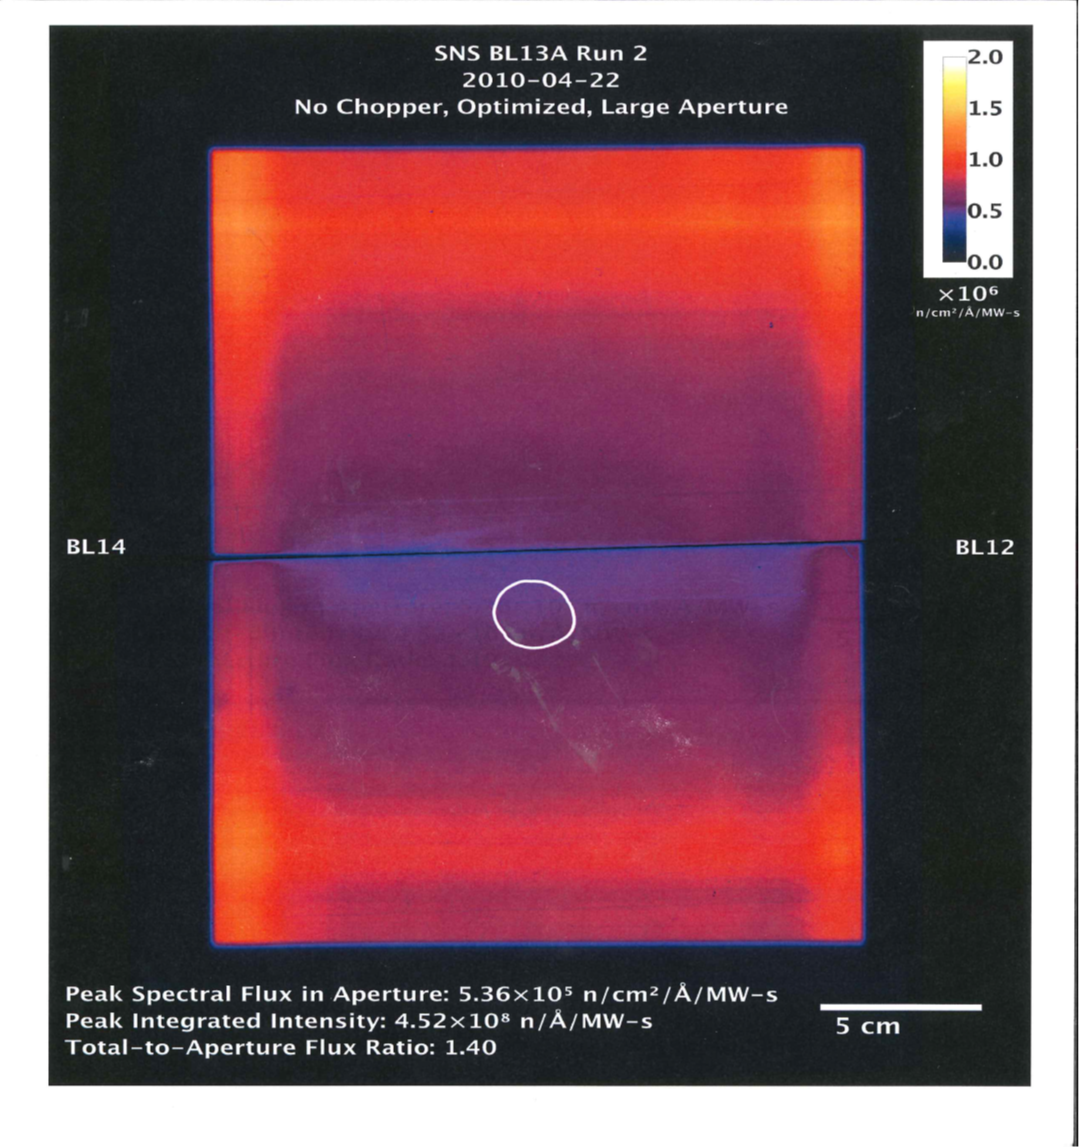
\includegraphics[width=\textwidth]{figures/appendix-figs/beamimageplate.png}
\caption{Image of the neutron beam profile taken in 2010 from the 13A neutron guide.}
\label{fig:beam_image}
\end{figure}

\begin{figure}[h!]
\centering
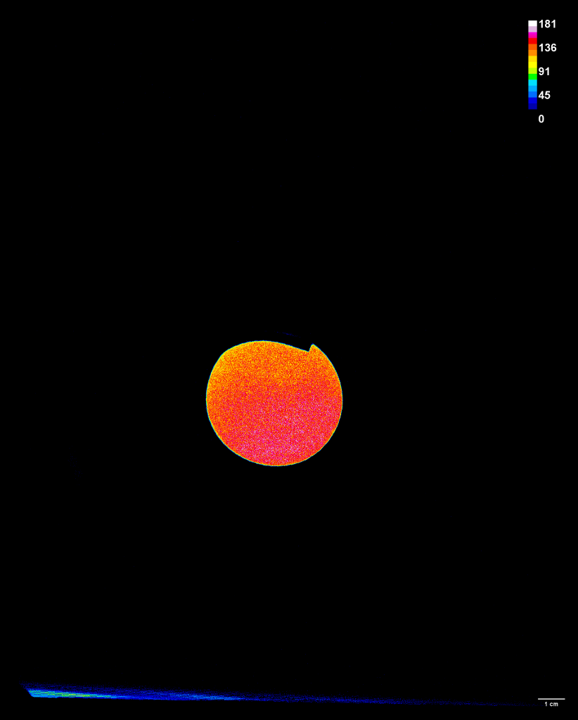
\includegraphics[width=\textwidth]{figures/appendix-figs/beforepol_beamimage.png}
\caption{Image of the neutron beam profile taken at the end of the BL-13A neutron flight tube.}
\label{fig:beam_image}
\end{figure}

\begin{figure}[h!]
\centering
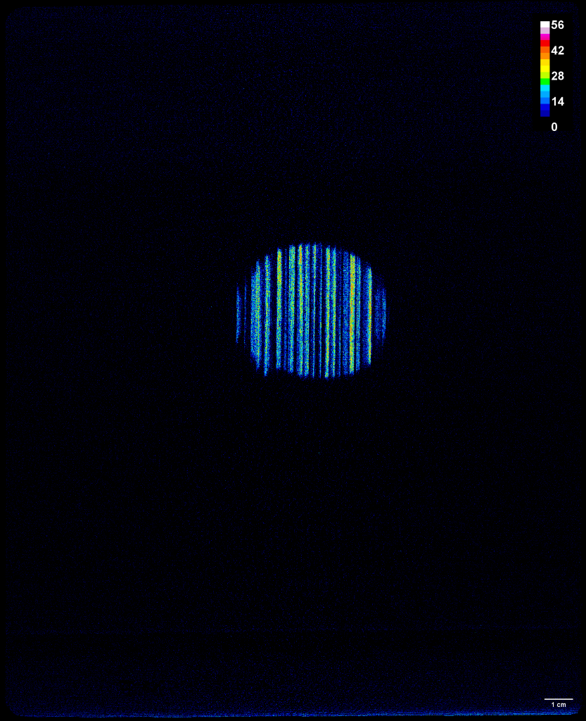
\includegraphics[width=\textwidth]{figures/appendix-figs/afterpol_beamimage.png}
\caption{Image of the neutron beam profile taken after the Super-mirror neutron polarizer.}
\label{fig:beam_image}
\end{figure}
